%% LyX 2.2.1 created this file.  For more info, see http://www.lyx.org/.
%% Do not edit unless you really know what you are doing.
\documentclass[english,12pt]{article}
\usepackage[T1]{fontenc}
\usepackage[latin9]{inputenc}
\usepackage{float}
\usepackage{mathtools}
\usepackage{amsmath}
\usepackage{amsthm}
\usepackage{amssymb}
\usepackage{graphicx}
\PassOptionsToPackage{normalem}{ulem}
\usepackage{ulem}

\makeatletter

%%%%%%%%%%%%%%%%%%%%%%%%%%%%%% LyX specific LaTeX commands.
\floatstyle{ruled}
\newfloat{algorithm}{tbp}{loa}
\providecommand{\algorithmname}{Algorithm}
\floatname{algorithm}{\protect\algorithmname}

%%%%%%%%%%%%%%%%%%%%%%%%%%%%%% Textclass specific LaTeX commands.
\theoremstyle{plain}
\newtheorem{thm}{\protect\theoremname}[section]
\theoremstyle{definition}
\newtheorem{defn}[thm]{\protect\definitionname}
\theoremstyle{plain}
\newtheorem{prop}[thm]{\protect\propositionname}
\ifx\proof\undefined
\newenvironment{proof}[1][\protect\proofname]{\par
\normalfont\topsep6\p@\@plus6\p@\relax
\trivlist
\itemindent\parindent
\item[\hskip\labelsep\scshape #1]\ignorespaces
}{%
\endtrivlist\@endpefalse
}
\providecommand{\proofname}{Proof}
\fi
\theoremstyle{plain}
\newtheorem{conjecture}[thm]{\protect\conjecturename}
\theoremstyle{definition}
\newtheorem{example}[thm]{\protect\examplename}
\theoremstyle{remark}
\newtheorem{rem}[thm]{\protect\remarkname}

%%%%%%%%%%%%%%%%%%%%%%%%%%%%%% User specified LaTeX commands.
\usepackage[margin=1in]{geometry}
\usepackage{todonotes}

\makeatother

\usepackage{babel}
\usepackage{listings}
\providecommand{\conjecturename}{Conjecture}
\providecommand{\definitionname}{Definition}
\providecommand{\examplename}{Example}
\providecommand{\propositionname}{Proposition}
\providecommand{\remarkname}{Remark}
\providecommand{\theoremname}{Theorem}
\renewcommand{\lstlistingname}{Listing}

\begin{document}

\title{Math 525: Lecture 25}

\date{April 17, 2018}

\maketitle
Last class, we saw that the identity
\begin{multline*}
\int_{[0,1]^{D}}f\equiv\int_{0}^{1}\cdots\int_{0}^{1}f(x_{1},\ldots,x_{D})dx_{1}\cdots dx_{D}=\mathbb{E}\left[f(X_{1},\ldots,X_{D})\right]\\
\text{where }X_{1},\ldots,X_{D}\sim U[0,1]\text{ independent and }f\text{ is Borel measurable}
\end{multline*}
yields a method (called the \emph{Monte Carlo method}) for computing
integrals: sample the function $N$ times to obtain observations $Y_{1},\ldots,Y_{N}\sim f(X_{1},\ldots,X_{D})$.
Then, compute
\[
\frac{S_{N}}{N}=\frac{Y_{1}+\cdots+Y_{N}}{N}
\]
which, by the law of large numbers, approximates $\mathbb{E}Y$.

\section{Computational effort of Monte Carlo}

Instead of Monte Carlo, consider approximating the integral using
Riemann sums:
\[
\int_{0}^{1}\cdots\int_{0}^{1}f(x_{1},\ldots,x_{D})dx_{1}\cdots dx_{D}\approx\sum_{1\leq i_{1},\ldots,i_{D}\leq N}f(i_{1}\Delta x,\ldots,i_{D}\Delta x)(\Delta x)^{D}\text{ where }\Delta x=N^{-1}.
\]
Note, in particular, that the function $f$ has to be evaluated $N^{D}$
times. This is referred to as the \emph{curse of dimensionality}:
for a given accuracy, we must increase the number of function evaluations
exponentially as the dimension increases. The same is true of other
``quadrature methods'' (e.g., trapezoid rule, Simpson's rule, etc.),
it does not apply only to Riemann sums.

The appeal of Monte Carlo is that unlike quadrature rules, it requires
only $N$ function evaluations to obtain $O(1/\sqrt{N})$ error (by
the CLT). Therefore, while Monte Carlo might be ill-suited for computing
low-dimensional integrals (e.g., $D=1$ or $D=2$), it is well-suited
to computing high-dimensional ones.

\section{Quasi-Monte Carlo}

\subsection*{Discrepancy}

Consider the two-dimensional ($D=2$) case. Sampling $Z\sim U([0,1]\times[0,1])$
using a uniform distribution $N=1000$ times, we obtain the following
scatter plot:

\begin{figure}[H]
\centering{}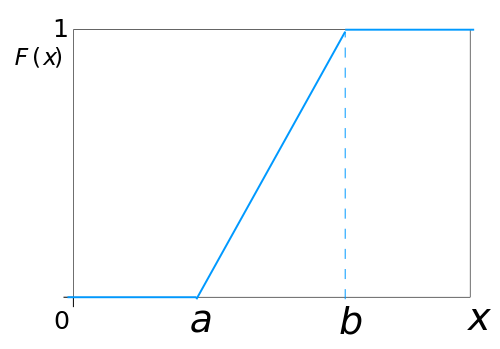
\includegraphics[width=5in]{uniform}
\end{figure}

In particular, there are regions of high density (lots of points)
and regions of low density (few points). In hopes of obtaining a better
error than $O(1/\sqrt{N})$, quasi-Monte Carlo uses instead a \uline{deterministic}
sequence $(z^{n})_{n}$ in $[0,1]^{D}$. This sequence is chosen to
have ``good density properties''. Then, the integral $\int_{[0,1]^{D}}f$
is approximated by
\[
\frac{1}{N}\sum_{n=1}^{N}f(z^{n})\equiv\frac{1}{N}\sum_{n=1}^{N}f(z_{1}^{n},\ldots,z_{D}^{n}).
\]
What does it mean for a sequence to have ``good density properties''?
One way to characterize this is through by discrepancy:
\begin{defn}
The \emph{discrepancy} of a nonempty set $P=\{z_{1},\ldots,z_{N}\}\subset[0,1]^{D}$
is
\[
d(P)=\sup_{\substack{0\leqslant a_{i}<b_{i}\leqslant1\\
i=1,\ldots,D
}
}\left|\prod_{i=1}^{D}(b_{i}-a_{i})-\frac{\left|P\cap\prod_{i=1}^{D}[a_{i},b_{i})\right|}{N}\right|.
\]
\end{defn}
This definition looks scarier than it is. Let's go over it carefully.
For some choice of endpoints $0\leq a_{i}<b_{i}\leq1$ ($i=1,\ldots D$),
let $A=\prod_{i=1}^{D}[a_{i},b_{i})$. Note that $A$ is just a ``hyper-rectangle''
in the hyper-cube $[0,1]^{D}$. Therefore, the product $\prod_{i=1}^{D}(b_{i}-a_{i})$
is nothing other than the volume of $A$. Moreover, the quantity $|P\cap A|$
is the number of points that are in $A$. Therefore, the discrepancy
corresponds to picking a hyper-rectangle that has the ``worst density''
with respect to the points $P=\{z_{1},\ldots,z_{n}\}$.
\begin{defn}
The \emph{star discrepancy }of a nonempty set $P=\{z_{1},\ldots,z_{N}\}\subset[0,1]^{D}$
is
\[
d^{*}(P)=\sup_{\substack{0<u_{i}\leqslant1\\
i=1,\ldots,D
}
}\left|\prod_{i=1}^{D}u_{i}-\frac{\left|P\cap\prod_{i=1}^{D}[0,u_{i})\right|}{N}\right|.
\]
\end{defn}
The star discrepancy is almost identical to the discrepancy: all that
differs is that we fix our attention to hyper-rectangles of the form
$\prod_{i=1}^{D}[0,u_{i})$.
\begin{prop}
For any nonempty finite set $P\subset[0,1]^{D}$, 
\[
d^{*}(P)\leq d(P)\leq2^{D}d^{*}(P).
\]
\end{prop}
\begin{proof}
The leftmost inequality is trivial. As for the rightmost inequality,
let's first consider the one-dimensional case ($D=1$). Note that
\[
[a,b)=[0,b)\setminus[0,a).
\]
Therefore,
\[
\left|P\cap[a,b)\right|=\left|P\cap\left([0,b)\setminus[0,a)\right)\right|=\left|P\cap[0,b)\right|-\left|P\cap[0,a)\right|.
\]
Putting this all together,
\begin{multline*}
d(P)=\sup_{0\leq a<b\leq1}\left|\left(b-a\right)-\frac{\left|P\cap[a,b)\right|}{N}\right|=\sup_{0\leq a<b\leq1}\left|\left(b-\frac{\left|P\cap[0,b)\right|}{N}\right)-\left(a-\frac{\left|P\cap[0,a)\right|}{N}\right)\right|\\
\leq\sup_{0<b\leq1}\left|b-\frac{\left|P\cap[0,b)\right|}{N}\right|+\sup_{0\leq a<1}\left|a-\frac{\left|P\cap[0,a)\right|}{N}\right|=d^{*}(P)+d^{*}(P)=2d^{*}(P).
\end{multline*}
The same idea extends to higher dimensions ($D>1$).
\end{proof}

\subsection*{Koksma\textendash Hlawka inequality}
\begin{prop}[Koksma\textendash Hlawka]
Let $P=\{z_{1},\ldots,z_{N}\}$ be a nonempty subset of $[0,1]^{D}$.
Then,
\[
\left|\frac{1}{N}\sum_{n=1}^{N}f(z^{n})-\int_{[0,1]^{D}}f\right|\leq V_{HK}(f)d^{*}(P)
\]
where $V_{HK}(f)$ is the Hardy\textendash Krause variation of $f$.
\end{prop}
The proof of this result (and even the definition of $V_{HK}(\cdot)$)
is far out of the scope of this class. However, we can interpret this
result as telling us that for any ``well-behaved'' function $f$,
the error in quasi-Monte Carlo using points $P=\{z_{1},\ldots,z_{N}\}$
is at most
\[
C_{f}d^{*}(P)
\]
where $C_{f}$ is some positive constant that depends only on $f$.

In other words, the quality of quasi-Monte Carlo depends only on the
(star) discrepancy of the sequence we choose. In particular, we would
like to pick the sequence to have the lowest (star) discrepancy possible.
We should mention at this point that it is not known what the lowest
possible (star) discrepancy is:
\begin{conjecture}
There is a constant $C_{D}$ depending only on the dimension $D$
such that
\[
d^{*}(P)\geq C_{D}\frac{\left(\ln N\right)^{D-1}}{N}
\]
for any nonempty set $P=\{z_{1},\ldots,z_{N}\}\subset[0,1]^{D}$.
\end{conjecture}
The conjecture has been verified for $D=1$ ($C_{1}=1/2$) and $D=2$
($C_{2}=\frac{1}{8}e^{W_{-1}(-\frac{1}{2e})+1}=0.0233352886063546\ldots$)
but remains open for $D\geq3$.

\subsection*{Van der Corput (and Halton) sequences}

The \emph{Van der Corput sequence} is a simple example of a \emph{low
discrepancy sequence}. It is a sequence in one dimension ($D=1$),
constructed as follows. Fix a base $b$. For a positive integer $n$,
let $n=(\cdots n_{1}n_{0})_{b}$ denote its base $b$ expansion (i.e.,
$0\leq n_{j}<b$ is the $j$-th digit of $n$ in base $b$). Then,
\[
n=n_{0}+n_{1}b+n_{2}b^{2}+\cdots
\]
The $n$-th element of the Van der Corput sequence is then given by
\[
\varphi_{b}(n)=n_{0}b^{-1}+n_{1}b^{-2}+n_{2}b^{-3}+\cdots
\]
In other words, the Van der Corput sequence ``reverses'' the base
$b$ expansion of the natural numbers.
\begin{example}
In $b=2$, note that $0=(0)_{2}$, $1=(1)_{2}$, $2=(10)_{2}$, $3=(11)_{2}$,
$4=(100)_{2}$, etc. Therefore, the Van der Corput sequence is
\[
\left\{ (0)_{2},(0.1)_{2},(0.01)_{2},(0.11)_{2},(0.001)_{2},\ldots\right\} .
\]
Converting these numbers back to base 10,
\[
\left\{ 0,0.5,0.25,0.75,0.125,\ldots\right\} .
\]
\end{example}
\begin{rem}
The Halton sequences generalize the Van der Corput sequences to $D>1$.
\end{rem}
The following is a slight generalization of Van der Corput's original
result (1935) due to S. Harber (1966):
\begin{prop}
Let $P=\{\varphi_{2}(0),\ldots,\varphi_{b}(N-1)\}$ be the first $N>1$
elements of the Van der Corput sequence in base $b=2$. Then,
\[
Nd^{*}(P)\leq\frac{1}{3}\log_{2}N+C
\]
for some $C>0$.
\end{prop}

\subsection*{Sobol sequences}

Probably the most popular low discrepancy sequence is the Sobol sequence.
I mention it here only so that you are aware of it by name. Figure
\ref{fig:sobol} shows the first 1000 points of the Sobol sequence
(compare with the 1000 uniform samples at the beginning of this lecture).

\begin{figure}
\begin{centering}
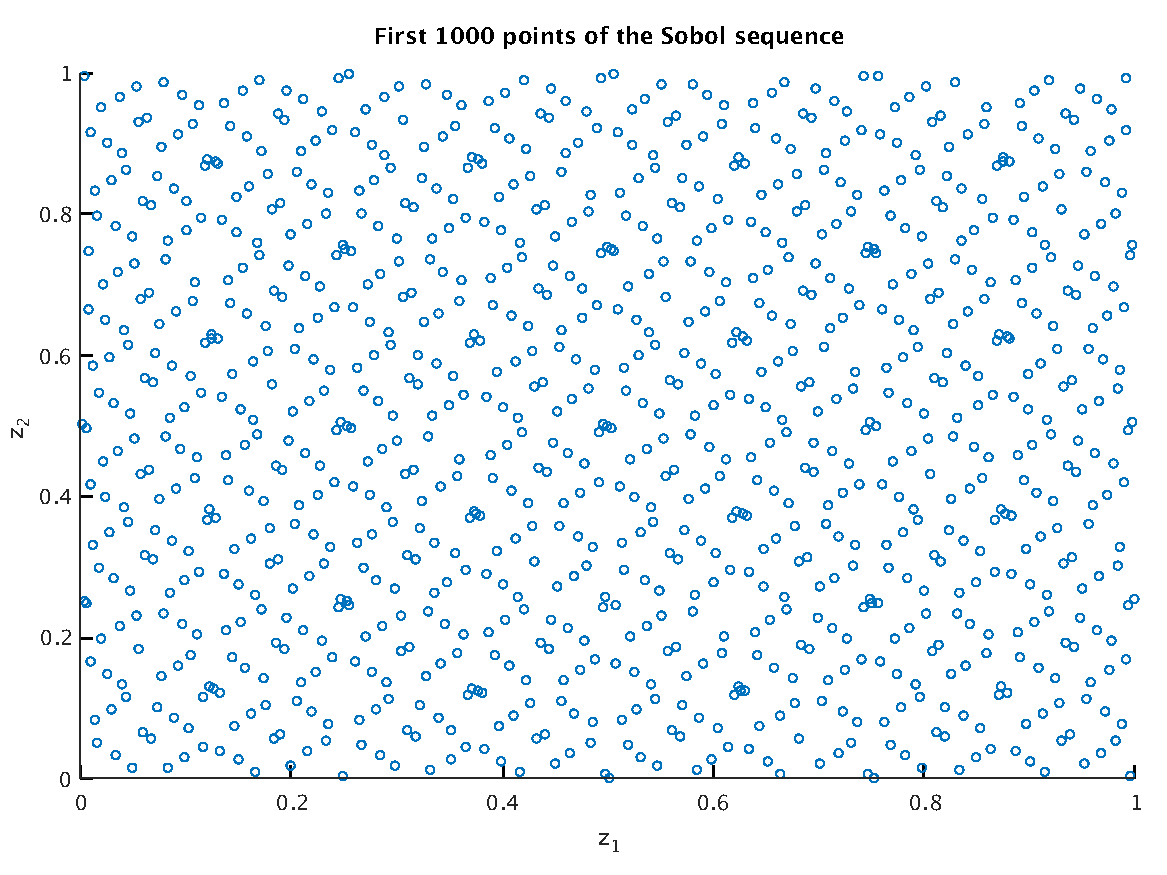
\includegraphics[width=5in]{sobol}
\par\end{centering}
\caption{2d Sobol sequence\label{fig:sobol}}
\end{figure}

Algorithm \ref{alg:pi} gives some C++ code to compute $\pi$ with
a two-dimensional Sobol sequence $(z^{n})_{n\geq1}$. Setting $N$
to be 10 million, we obtain $\pi\approx3.1415952$ (much more accurate
than the plain Monte Carlo approach we saw last class).

\begin{algorithm}
\begin{lstlisting}[language={C++},basicstyle={\scriptsize}]
#include <iomanip>
#include <iostream>

// http://people.sc.fsu.edu/~jburkardt/cpp_src/sobol/sobol.html
#include "sobol.hpp"

int main()
{
	const int N         = 10000000;
	long long int seed  = 1;
	long long int count = 0;

	double r[2];
	for(int n = 0; n < N; ++n)
	{
		i8_sobol(2, &seed, r);
		const bool inside_circle = r[0] * r[0] + r[1] * r[1] <= 1.;
		if(inside_circle) { ++count; }
	}

	const double pi_approximate = 4. * ((double) count) / N;
	std::cout << std::setprecision(16) << pi_approximate << std::endl;

	return 0;
}
\end{lstlisting}

\caption{quasi-Monte Carlo method to approximate $\pi$\label{alg:pi}}
\end{algorithm}

\end{document}
